\renewcommand{\headrulewidth}{0pt}
\thispagestyle{empty}
\rotatebox{90}{%
\noindent
\vbox to\textwidth{%
\vfill\hbox to\textheight{\hfill\begin{tabular}{c}
\includegraphics{figures/prelim_01.png}\\
{\kan{\textbf{ಗಂಗಾಧರ ಭಟ್ಟರ ಮನೆ ದೇವರು \enginline{-} ಮಾರುತಿ ಸನ್ನಿಧಾನ}}}
\end{tabular}\hfill}
\vfill}}

\eject
\thispagestyle{empty}

\rotatebox{90}{%
\noindent
\vbox to\textwidth{%
\vfill
\hbox to\textheight{\hfill\begin{tabular}{c}
\includegraphics{figures/prelim_03.png}\\
{\kan{\textbf{ವಿ ॥ ಗಂಗಾಧರ ಭಟ್ಟರ ಮಾತಾ\enginline{-}ಪಿತೃಗಳು\enginline{-}ಶ್ರೀಮತಿ ರೇವತಮ್ಮ ಮತ್ತು  ವೇ ॥ ಬ್ರ ॥ ಶ್ರೀ ವಿಘ್ನೇಶ್ವರ ಭಟ್ಟರು}}}
\end{tabular}\hfill}
\vfill}}

\eject

\thispagestyle{empty}
\rotatebox{90}{%
\noindent
\vbox to\textwidth{%
\vfill
\hbox to\textheight{\hfill\begin{tabular}{c}
\includegraphics{figures/prelim_02.png}\\
{\kan{\textbf{ವಿ ॥ ಗಂಗಾಧರ ಭಟ್ಟರ ಗುರುಗಳು\enginline{-}ಮಹಾಮಹೋಪಾಧ್ಯಾಯ ಎನ್.ಎಸ್.ರಾಮಭದ್ರಾಚಾರ್ಯ ದಂಪತಿಗಳು}}}
\end{tabular}\hfill}
\vfill}}

\input src/partI/invitation
\input src/partI/news_paper_cuttings

\eject

\begin{center}
{\Huge ಅಭಿವಂದನ ಕಾರ್ಯಕ್ರಮದ ಭಾವಚಿತ್ರಗಳು}
\addcontentsline{toc}{chapter}{\protect\numberline{6}ಅಭಿವಂದನ ಕಾರ್ಯಕ್ರಮದ ಭಾವಚಿತ್ರಗಳು}
\end{center}
\smallskip

\thispagestyle{empty}
{\tabcolsep=0pt
\noindent
\begin{tabular}{>{\centering}p{11cm}}
\includegraphics[scale=0.82]{figures/02.png}\\
\textbf{ ಶ್ರೀಗಂಗಾಧರ ಭಟ್ಟರು ಅಧ್ಯಯನ ಮತ್ತು ಅಧ್ಯಾಪನ ಮಾಡಿದ\\ ಮಹಾರಾಜಸಂಸ್ಕೃತ ಮಹಾಪಾಠಶಾಲೆ}\\[12pt]
\includegraphics[scale=0.75]{figures/01.png}\\
\textbf{ ಮಹಾರಾಜಸಂಸ್ಕೃತ ಮಹಾಪಾಠಶಾಲೆಯ ಸರಸ್ವತೀಪ್ರಾಸಾದದ ದ್ವಾರ}
\end{tabular}
}
\eject


\thispagestyle{empty}

{\tabcolsep=0pt
\noindent
\begin{tabular}{>{\centering}p{11cm}}
\includegraphics{figures/06.png}\\
\textbf{ ಶ್ರೀಯುತರನ್ನು ಬರಮಾಡಿಕೊಳ್ಳಲು ಮಹಾದ್ವಾರದಲ್ಲಿ ಕಾತರಿಸುತ್ತಿರುವ  ಶಿಷ್ಯವೃಂದ}\\[20pt]
\includegraphics{figures/08.png}\\
\textbf{ವಾಹನದಲ್ಲಿ ಆಗಮಿಸುತ್ತಿರುವ ಶ್ರೀಗಂಗಾಧರ ಭಟ್ಟ ದಂಪತಿಗಳು}
\end{tabular}
}

\eject
\thispagestyle{empty}

{\tabcolsep=0pt
\noindent
\begin{tabular}{>{\centering}p{11cm}}
\includegraphics{figures/09.png}\\
\textbf{ಶ್ರೀಯುತರಿಗೆ ಪೂರ್ಣಕುಂಭ ಸ್ವಾಗತ}\\[20pt]
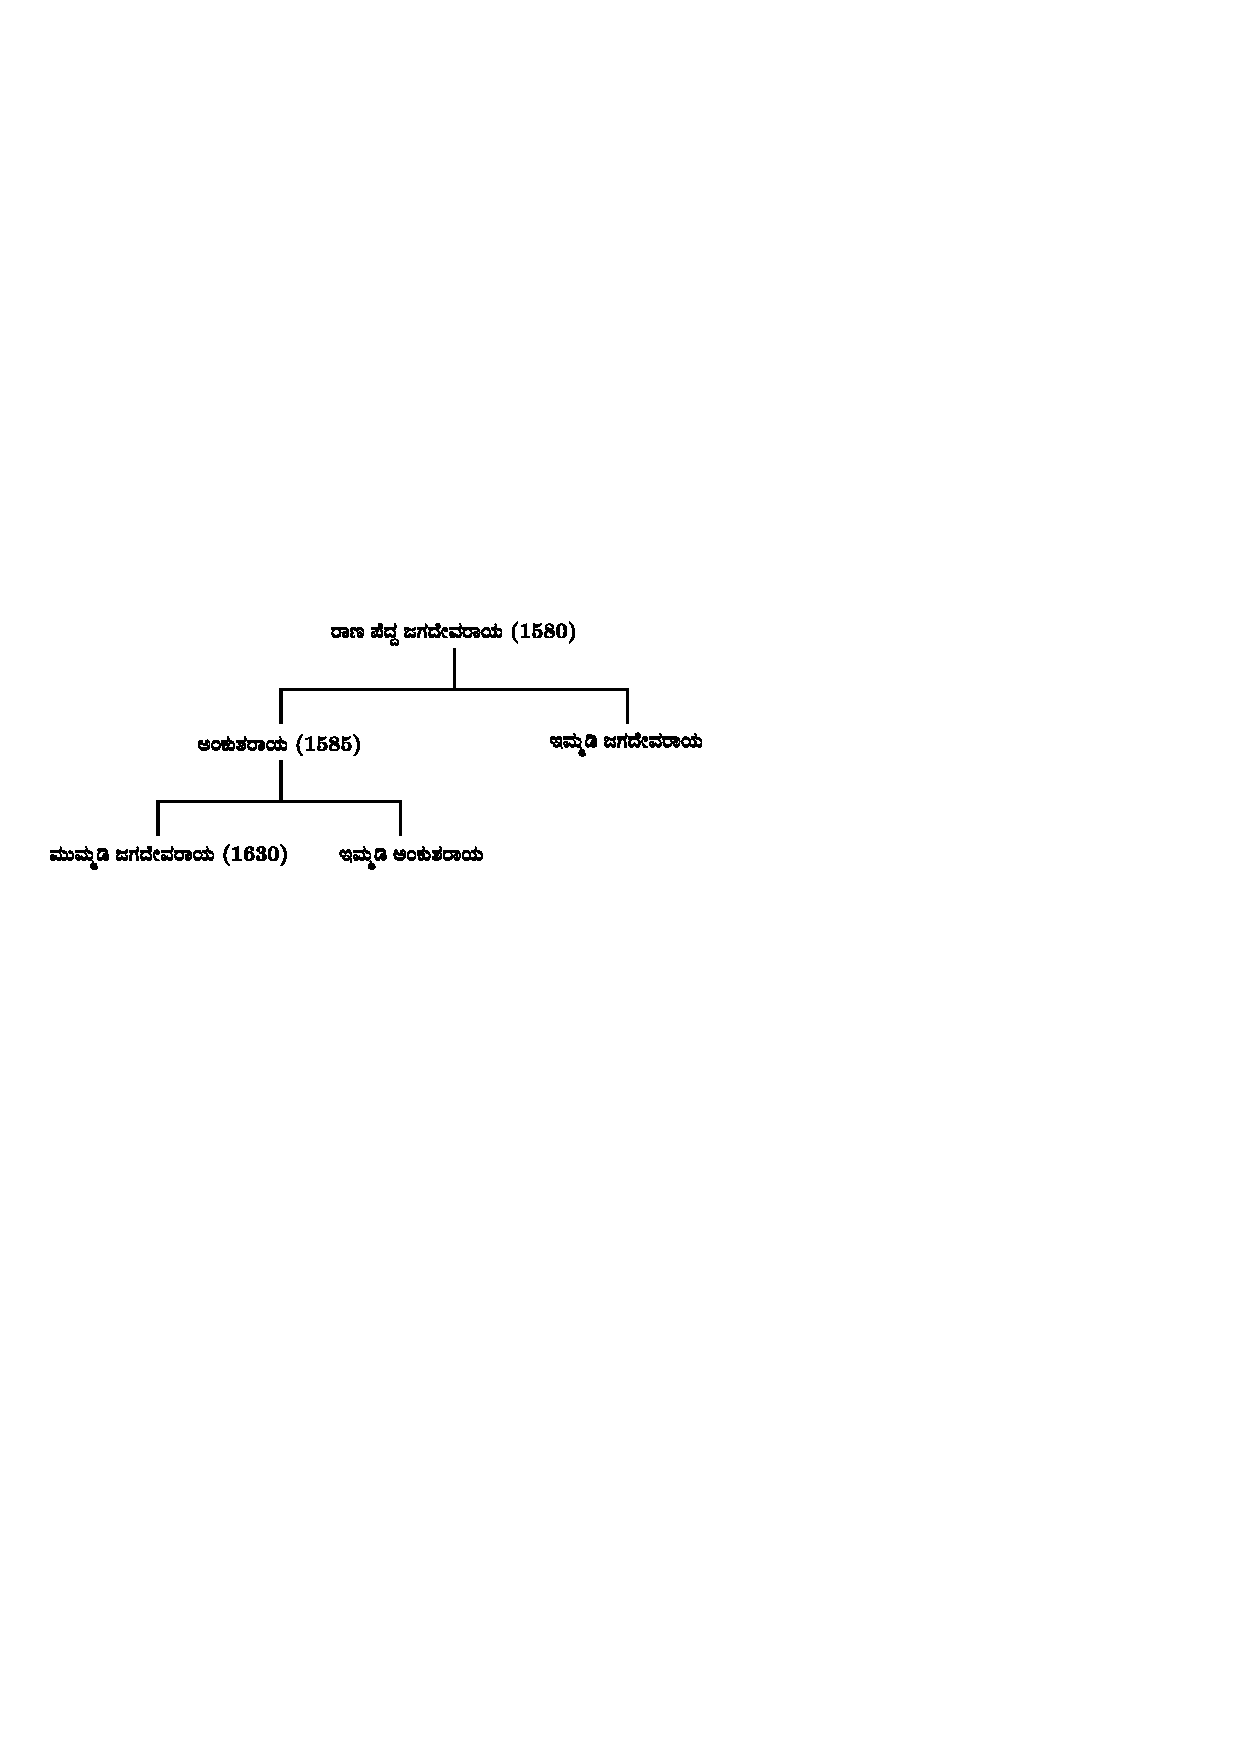
\includegraphics{figures/10.png}\\
\textbf{ವೇದಸ್ವಸ್ತಿಯೊಂದಿಗೆ ಶುಭಾಗಮನ}
\end{tabular}
}

\eject
\thispagestyle{empty}

{\tabcolsep=0pt
\noindent
\begin{tabular}{>{\centering}p{11cm}}
\includegraphics{figures/05.png}\\
\textbf{ಸರಸ್ವತೀಪ್ರಾಸಾದದಲ್ಲಿರುವ ವಿದ್ಯಾಗಣಪತಿ ಮಹಾಸನ್ನಿಧಾನ ದರ್ಶನ}\\[20pt]
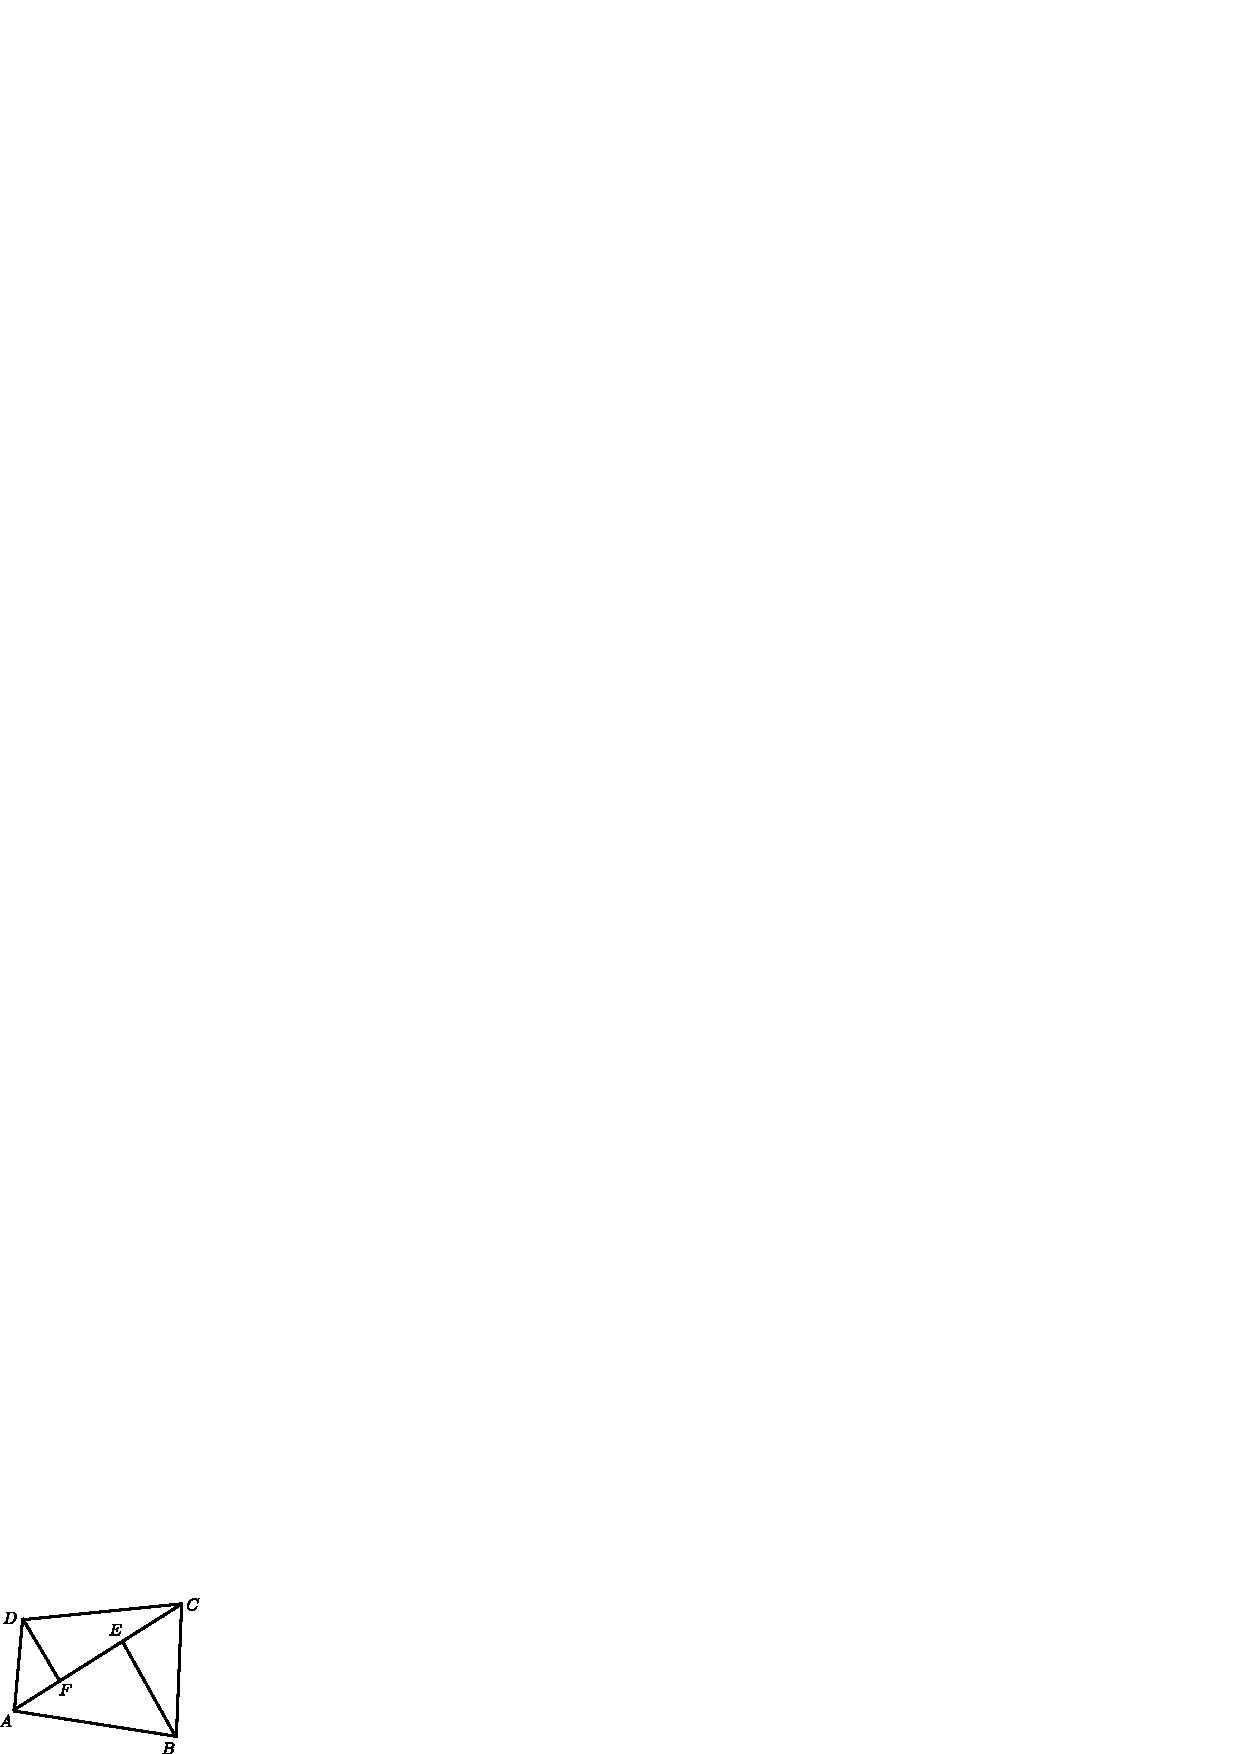
\includegraphics{figures/11.png}\\
\textbf{ ಮಂಗಳಾರತಿ ಸ್ವೀಕಾರ}
\end{tabular}
}

\eject
\thispagestyle{empty}

{\tabcolsep=0pt
\noindent
\begin{tabular}{>{\centering}p{11cm}}
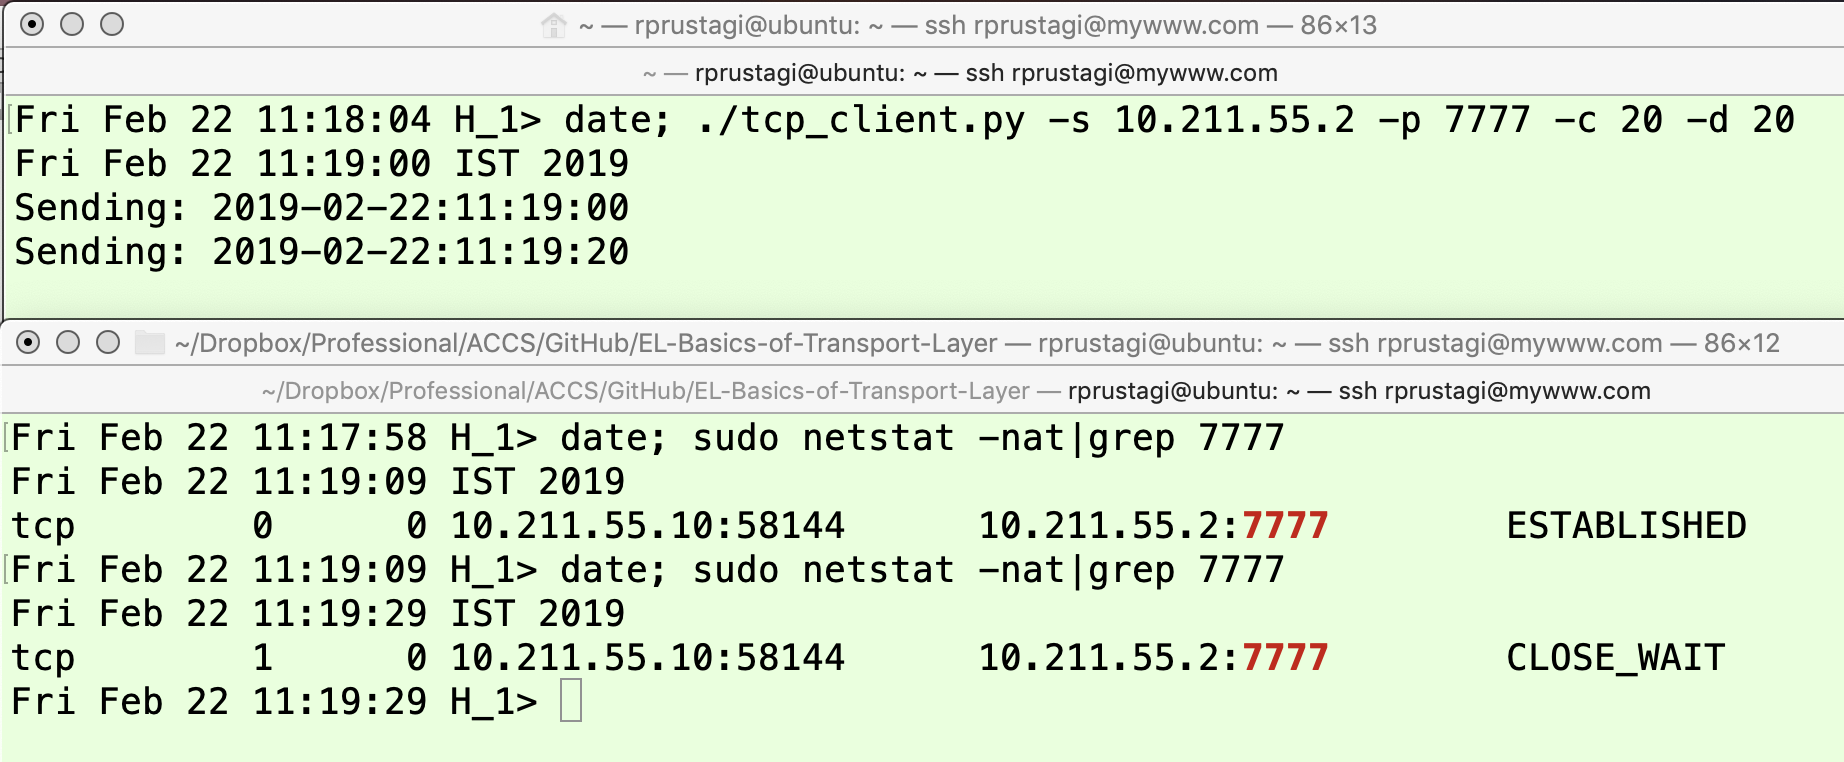
\includegraphics{figures/12.png}\\
\textbf{ದೀಪಪ್ರಜ್ವಾಲನಪೂರ್ವಕ ಕಾರ್ಯಕ್ರಮದ ಉದ್ಘಾಟನೆ - ವಿ ॥ ರಾಜೇಶ್ವರ ಶಾಸ್ತ್ರಿಗಳಿಂದ}\\[20pt]
\includegraphics{figures/13a.png}\\
\textbf{ವಿ ॥ಗಂಗಾಧರ ಭಟ್ಟರಿಂದ ದೀಪಪ್ರಜ್ವಾಲನೆ}
\end{tabular}
}

\eject
\thispagestyle{empty}
{\tabcolsep=0pt
\noindent
\begin{tabular}{>{\centering}p{11cm}}
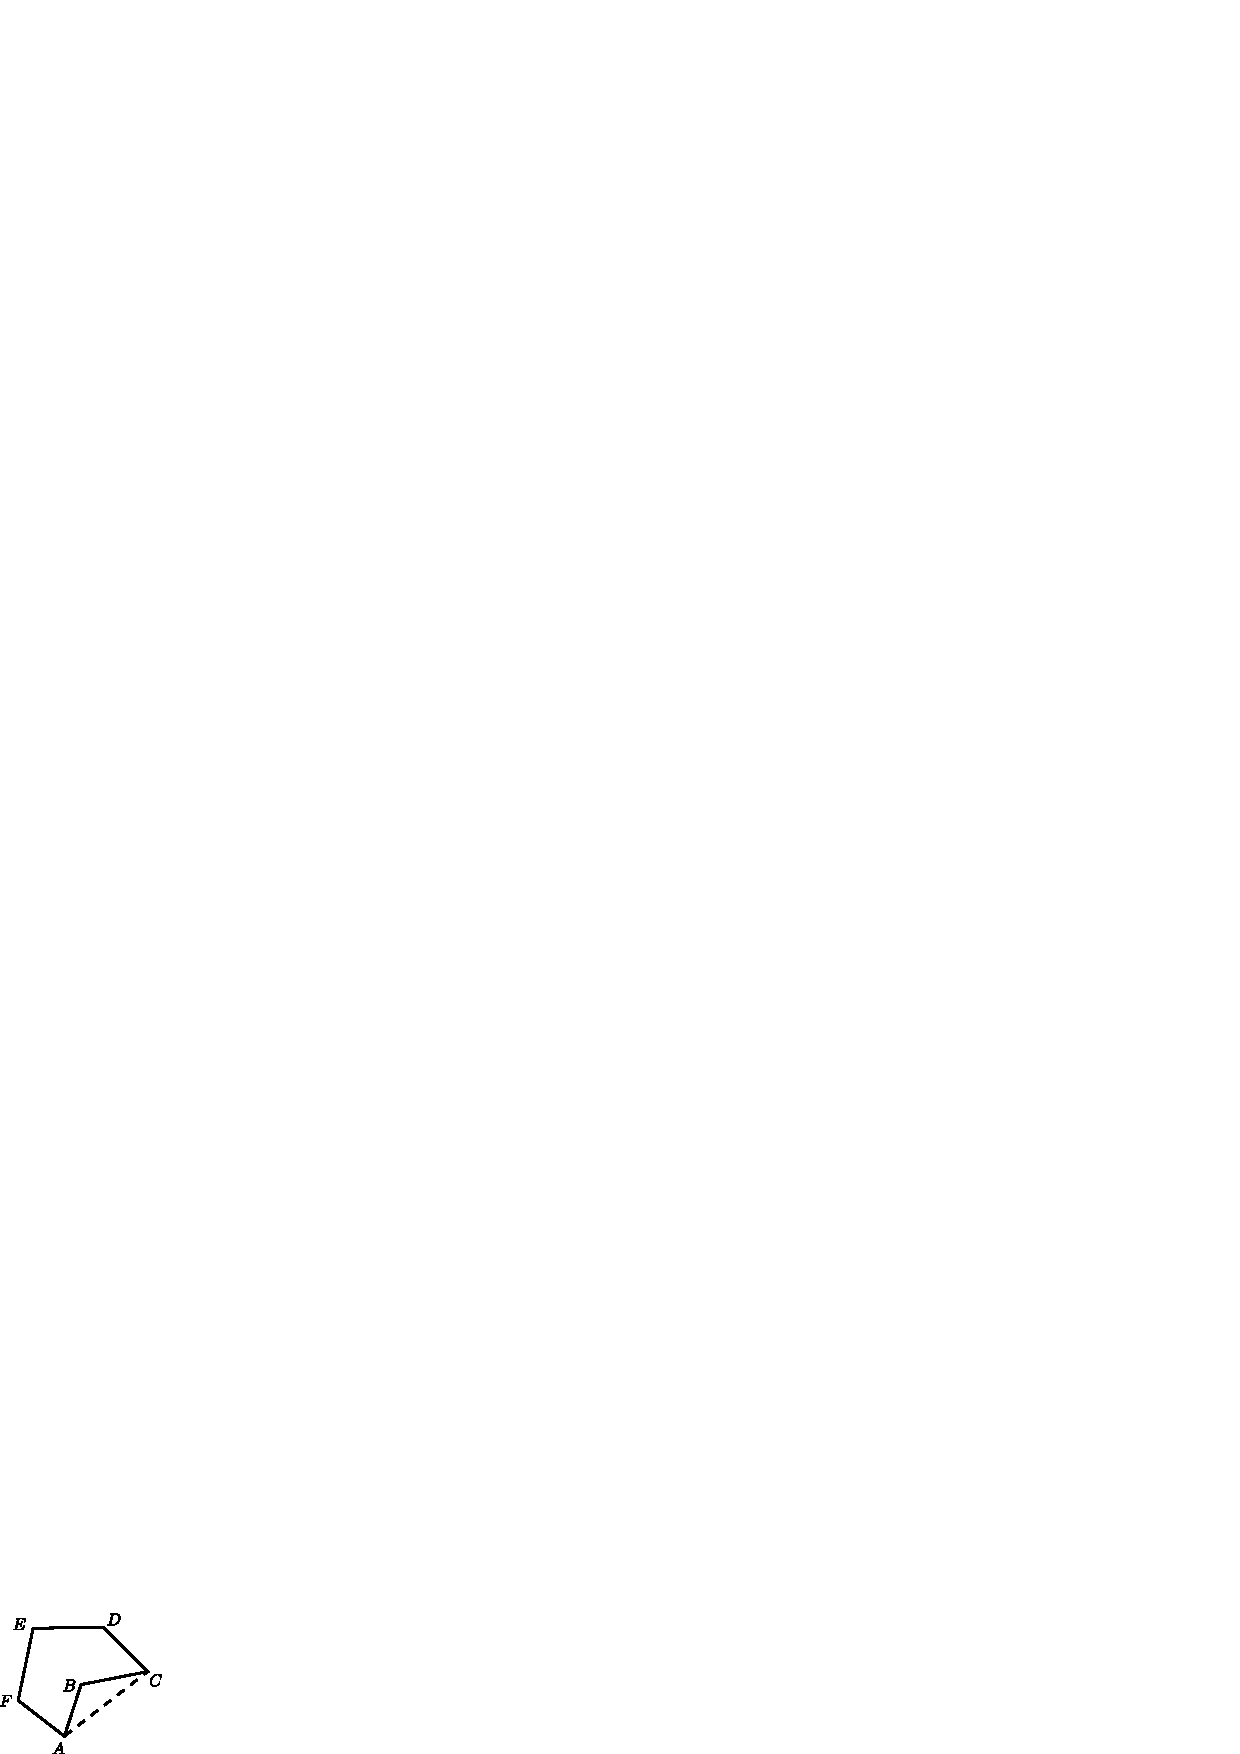
\includegraphics[scale=0.9]{figures/13.png}\\
\textbf{ಶ್ರೀಯುತರಿಗೆ ಸಮರ್ಪಿಸಲು  ಸಿದ್ಧಪಡಿಸಿರುವ ಶ್ರೀಯುತ ರಾಮಭದ್ರಾಚಾರ್ಯ\\ ದಂಪತಿಗಳ ಭಾವಚಿತ್ರ}\\[20pt]
\includegraphics[scale=0.9]{figures/28a.png}\\
\textbf{ಶ್ರೀಗಣಪತಿಸಚ್ಚಿದಾನಂದ ಆಶ್ರಮದ ವತಿಯಿಂದ\\ ಶ್ರೀಯುತರಿಗೆ ವಿ ॥ ವಂಶೀಕೃಷ್ಣರಿಂದ ಗೌರವ ಸಮರ್ಪಣೆ}
\end{tabular}
}



\eject
\thispagestyle{empty}

{\tabcolsep=0pt
\noindent
\begin{tabular}{>{\centering}p{11cm}}
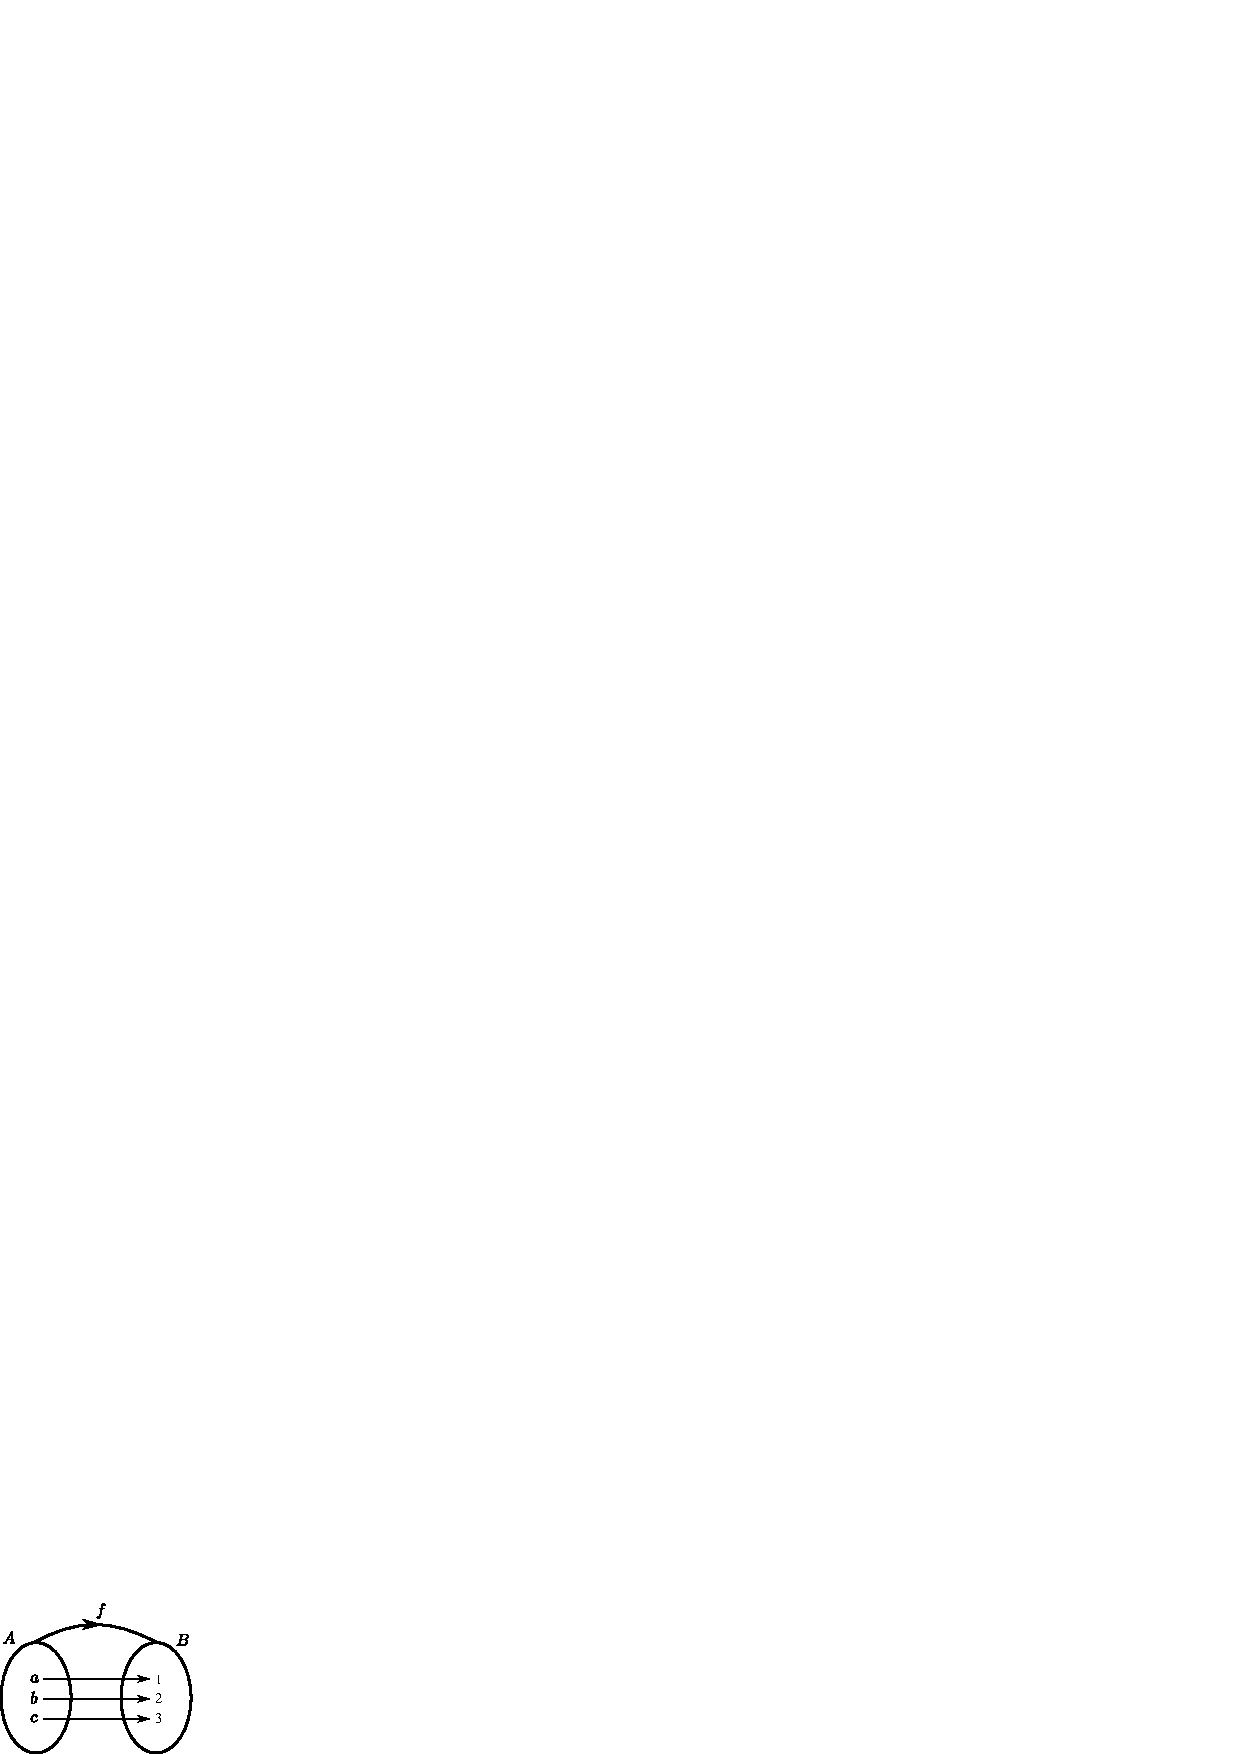
\includegraphics{figures/14.png}\\
\textbf{ವಾಕ್ಯಾರ್ಥಗೋಷ್ಠಿಯಲ್ಲಿ ಅಸೀನರಾಗಿರುವ ವಿದ್ವಾಂಸರು}\\[20pt]
\includegraphics{figures/14a.png}\\
\textbf{ವಾಕ್ಯಾರ್ಥಗೋಷ್ಠಿಯಲ್ಲಿ ಮಂಡಿಸಿರುವ ವಿದ್ವಾಂಸರು}\\[20pt]
\end{tabular}
}

\eject
\thispagestyle{empty}

{\tabcolsep=0pt
\noindent
\begin{tabular}{>{\centering}p{11cm}}
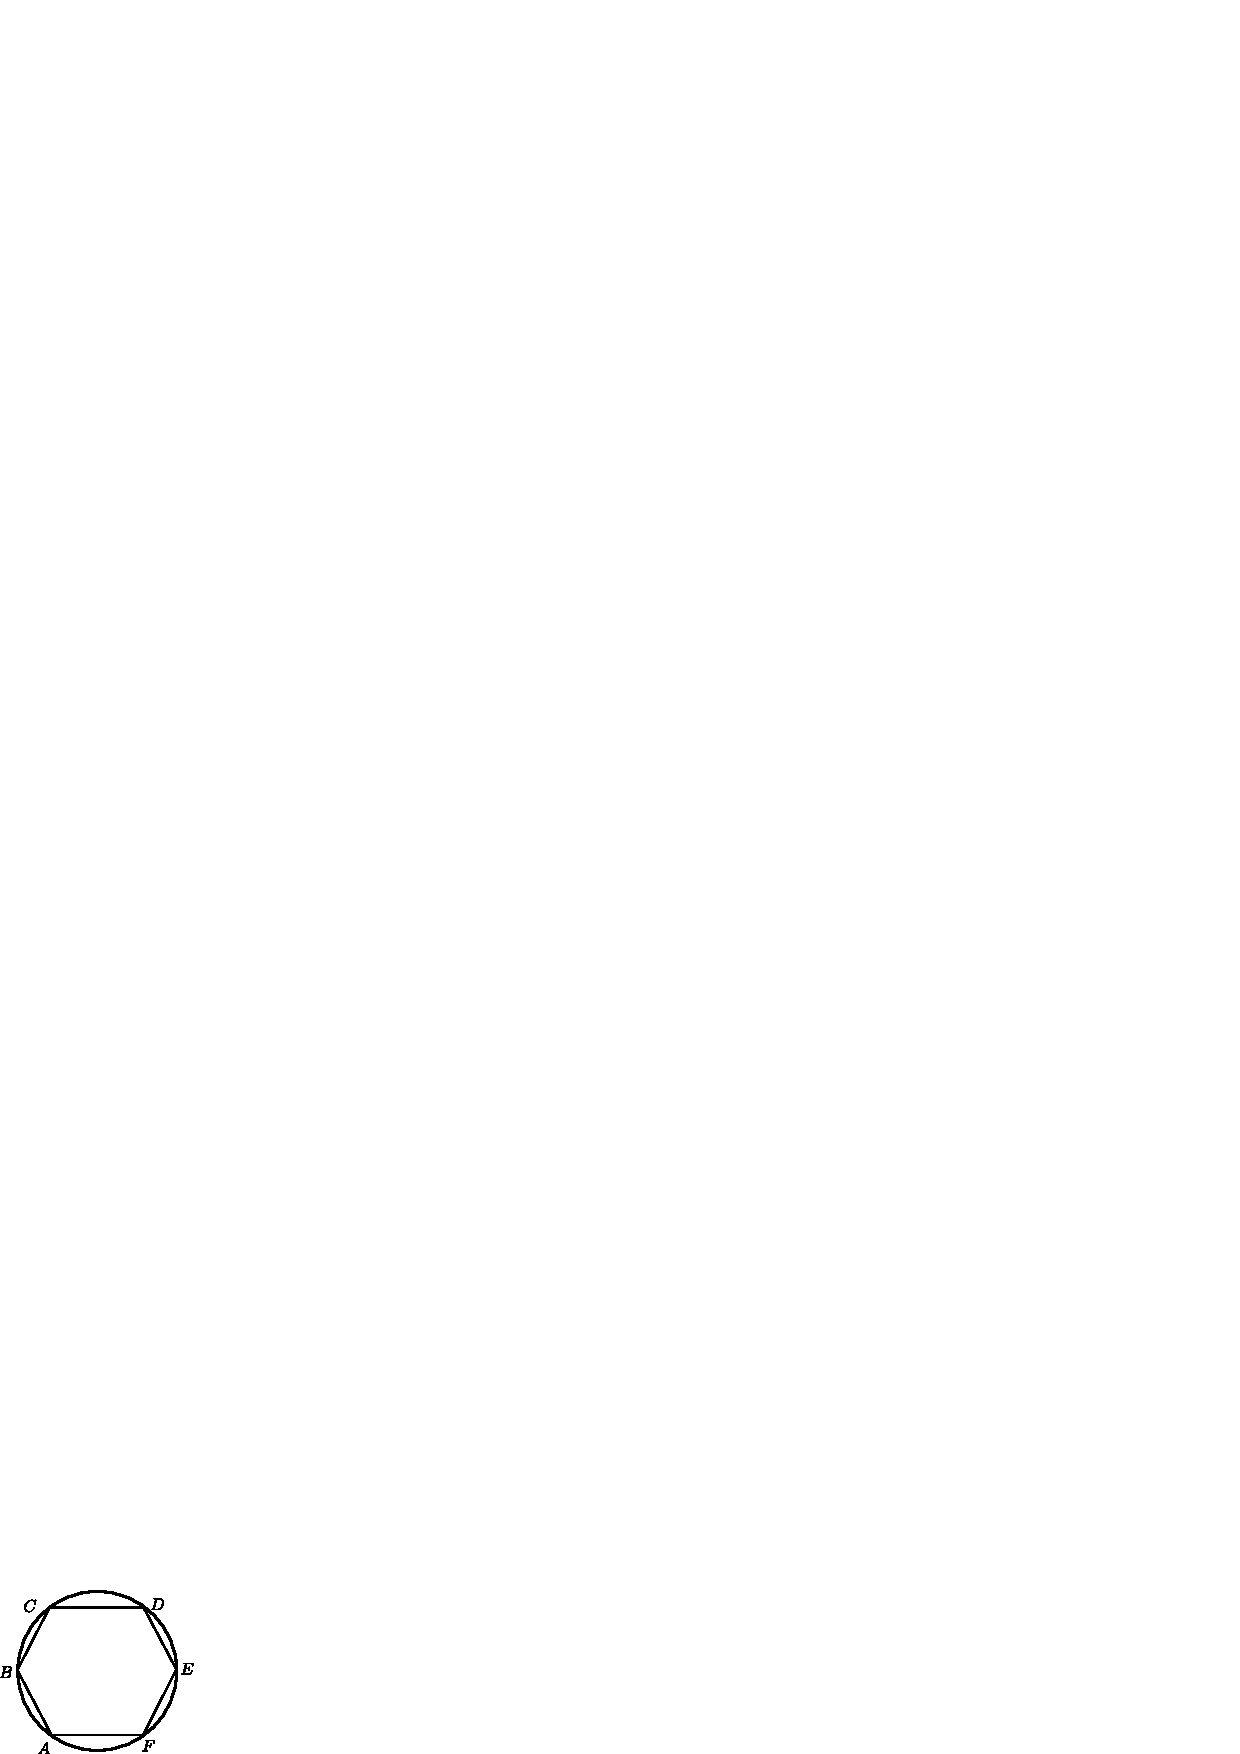
\includegraphics{figures/15.png}\\
\textbf{ಗಂಗಾಧರ ಭಟ್ಟರ ವಿದ್ಯಾರ್ಥೀ - ವಿ ॥ ಶಿವರಾಮರಿಂದ ವಾಕ್ಯಾರ್ಥ}\\[20pt]
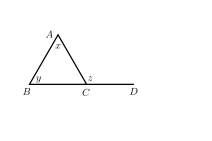
\includegraphics{figures/16.png}\\
\textbf{ಗಂಗಾಧರ ಭಟ್ಟರ ವಿದ್ಯಾರ್ಥೀ - ವಿ ॥ ಕೆ.ಎಲ್. ರಾಘವರಿಂದ ವಾಕ್ಯಾರ್ಥ}
\end{tabular}
}

\eject
\thispagestyle{empty}

{\tabcolsep=0pt
\noindent
\begin{tabular}{>{\centering}p{11cm}}
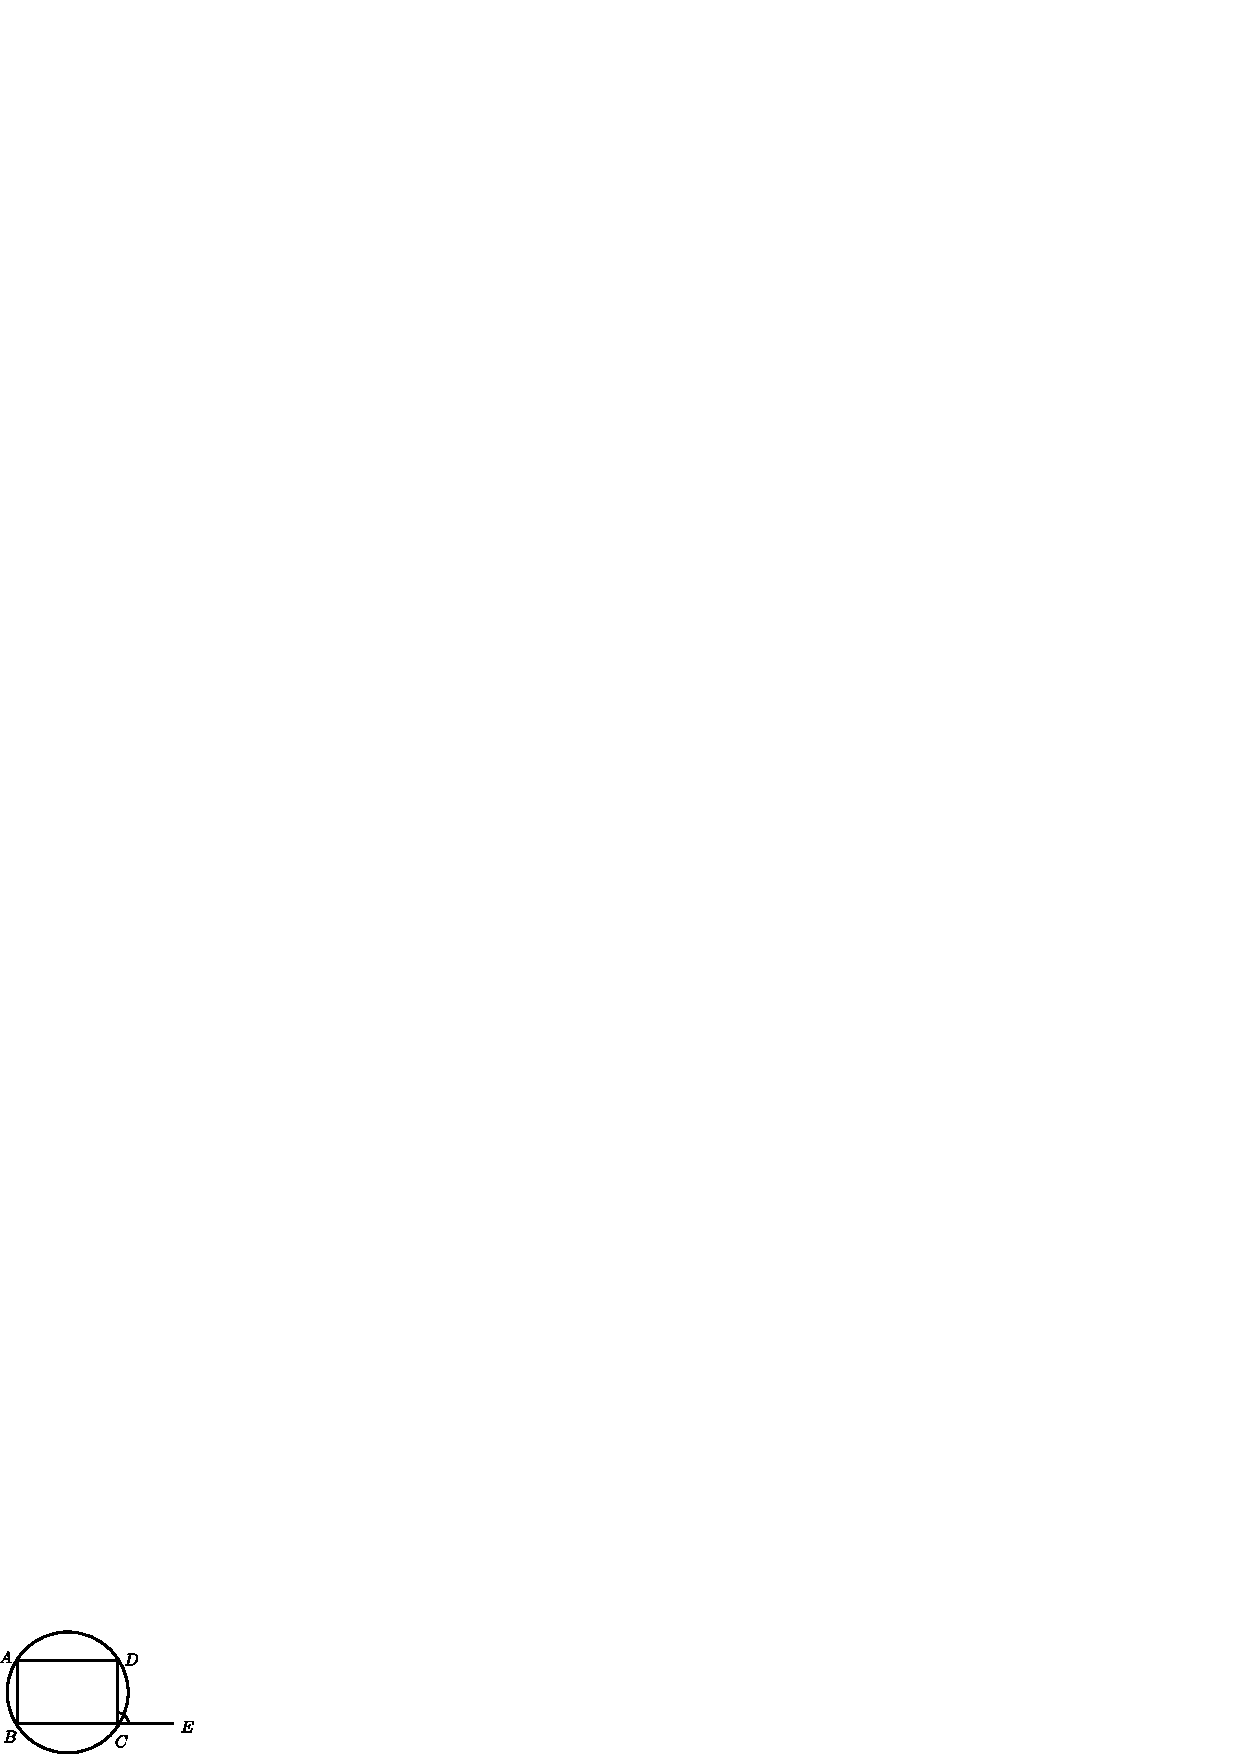
\includegraphics{figures/17.png}\\
\textbf{ವಾಕ್ಯಾರ್ಥಗೋಷ್ಠಿಯ ಅಧ್ಯಕ್ಷರಾದ ವಿ ॥ ರಾಜೇಶ್ವರ ಶಾಸ್ತ್ರಿಗಳಿಗೆ ಗೌರವ ಪ್ರದಾನ} \\[20pt]
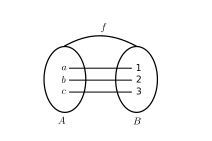
\includegraphics{figures/18.png}\\
\textbf{ರಾಜಮಾತೆ ಡಾ ॥` ಪ್ರಮೋದಾ ದೇವಿಯವರಿಗೆ ಪೂರ್ಣಕುಂಭ ಸ್ವಾಗತ}
\textbf{ರಾಜಮಾತೆ ಡಾ ॥ ಪ್ರಮೋದಾ ದೇವಿಯವರಿಗೆ ಪೂರ್ಣಕುಂಭ ಸ್ವಾಗತ}
\end{tabular}
}

\eject
\thispagestyle{empty}

{\tabcolsep=0pt
\noindent
\begin{tabular}{>{\centering}p{11cm}}
\includegraphics{figures/18a.png}\\
\textbf{ವಿದ್ಯಾಗಣಪತಿ ಸನ್ನಿಧಿಯೆಡೆಗೆ \\ ರಾಜಮಾತೆ ಡಾ ॥ ಪ್ರಮೋದಾ ದೇವಿಯವರ ಶುಭಾಗಮನ}\\[20pt]
\includegraphics{figures/18b.png}\\
\textbf{ವಿದ್ಯಾಗಣಪತಿ ಸನ್ನಿಧಿ}
\end{tabular}
}

\eject
\thispagestyle{empty}

{\tabcolsep=0pt
\noindent
\begin{tabular}{>{\centering}p{11cm}}
\includegraphics[scale=0.85]{figures/18c.png}\\
\textbf{ವಿದ್ಯಾಗಣಪತಿ ಸನ್ನಿಧಿಯಲ್ಲಿ ರಾಜಮಾತೆ ಪ್ರಮೋದಾ ದೇವಿಯವರು \\ವಿ ॥ ಗಂಗಾಧರ ಭಟ್ಟರು, ಡಾ ॥ ಪಿ.ಎನ್.ಶಾಸ್ತ್ರಿಗಳು ಮತ್ತು ಗಣ್ಯರು}\\[20pt]
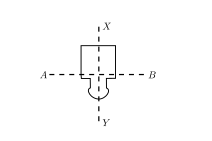
\includegraphics[scale=0.85]{figures/19.png}\\
\textbf{ ವಿ ॥ ಗಂಗಾಧರ ಭಟ್ಟರು, ಅವರ ಬಲಭಾಗದಲ್ಲಿ ರಾಜಮಾತೆಯವರು, ಅವರ ಪಕ್ಕದಲ್ಲಿ\\ಡಾ ॥ ಪಿ. ಎನ್. ಶಾಸ್ತ್ರಿಗಳು, ಅನಂತರ ಡಾ ॥ ನಿರಂಜನ ವಾನಳ್ಳಿಯವರು, ಪಕ್ಕದಲ್ಲಿ\\ವಿ ॥ ರಾ.\ ಶಾಸ್ತ್ರಿಗಳು. ಭಟ್ಟರ ಎಡಪಾರ್ಶ್ವದಲ್ಲಿ  ವಿ ॥ ಉಮಾಕಾಂತ ಭಟ್ಟರು}
\end{tabular}
}

\eject
\thispagestyle{empty}

{\tabcolsep=0pt
\noindent
\begin{tabular}{>{\centering}p{11cm}}
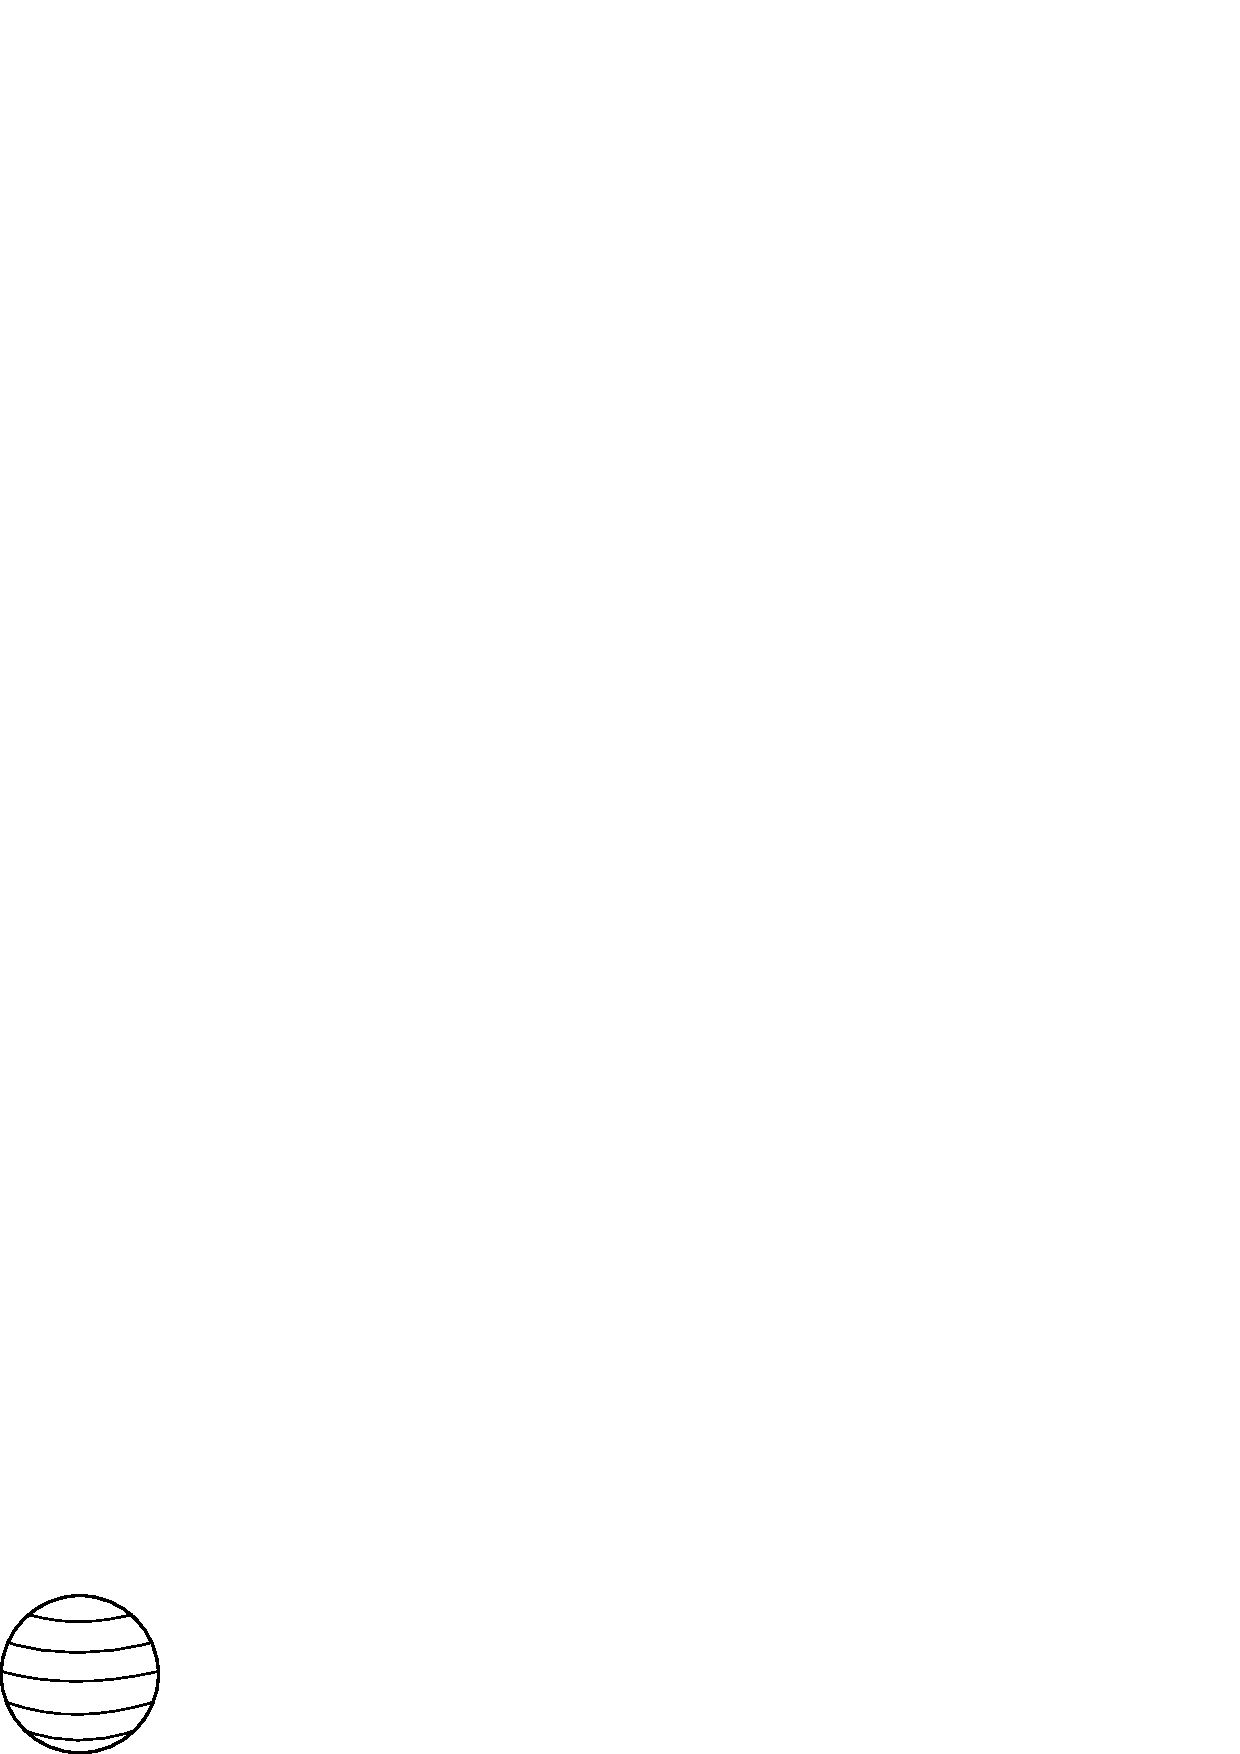
\includegraphics{figures/20.png}\\
\textbf{ಸಭೆಯಲ್ಲಿ  ಆಸೀನರಾಗಿರುವ ಅಭಿಮಾನಿ ಸಮೂಹ}\\[20pt]
\includegraphics{figures/20a.png}\\
\textbf{ಸಭೆಯಲ್ಲಿ  ಆಸೀನರಾಗಿರುವ ಅಭಿಮಾನಿ ಸಮೂಹ}
\end{tabular}
}

\eject
\thispagestyle{empty}

{\tabcolsep=0pt
\noindent
\begin{tabular}{>{\centering}p{11cm}}
\includegraphics{figures/20b.png}\\
\textbf{ಸಭೆಯಲ್ಲಿ  ಆಸೀನರಾಗಿರುವ ಅಭಿಮಾನಿ ಸಮೂಹ}\\[20pt]
\includegraphics{figures/20c.png}\\
\textbf{ಸಭೆಯಲ್ಲಿ  ಆಸೀನರಾಗಿರುವ ಅಭಿಮಾನಿ ಸಮೂಹ}
\end{tabular}
}

\eject
\thispagestyle{empty}

{\tabcolsep=0pt
\noindent
\begin{tabular}{>{\centering}p{11cm}}
\includegraphics{figures/20d.png}\\
\textbf{ಸಭೆಯಲ್ಲಿ  ಆಸೀನರಾಗಿರುವ ಅಭಿಮಾನಿ ಸಮೂಹ}\\[20pt]
\includegraphics{figures/20e.png}\\
\textbf{ಸಭೆಯಲ್ಲಿ  ಆಸೀನರಾಗಿರುವ ಅಭಿಮಾನಿ ಸಮೂಹ}
\end{tabular}
}


\eject
\thispagestyle{empty}

{\tabcolsep=0pt
\noindent
\begin{tabular}{>{\centering}p{11cm}}
\includegraphics{figures/21a.png}\\
\textbf{ಸಭೆಯಲ್ಲಿ  ಆಸೀನರಾಗಿರುವ ಅಭಿಮಾನಿ ಸಮೂಹ}\\[20pt]
\includegraphics{figures/20g.png}\\
\textbf{ವಿಶಾಲ ಸಭೆ}
\end{tabular}
}

\eject
\thispagestyle{empty}

{\tabcolsep=0pt
\noindent
\begin{tabular}{>{\centering}p{11cm}}
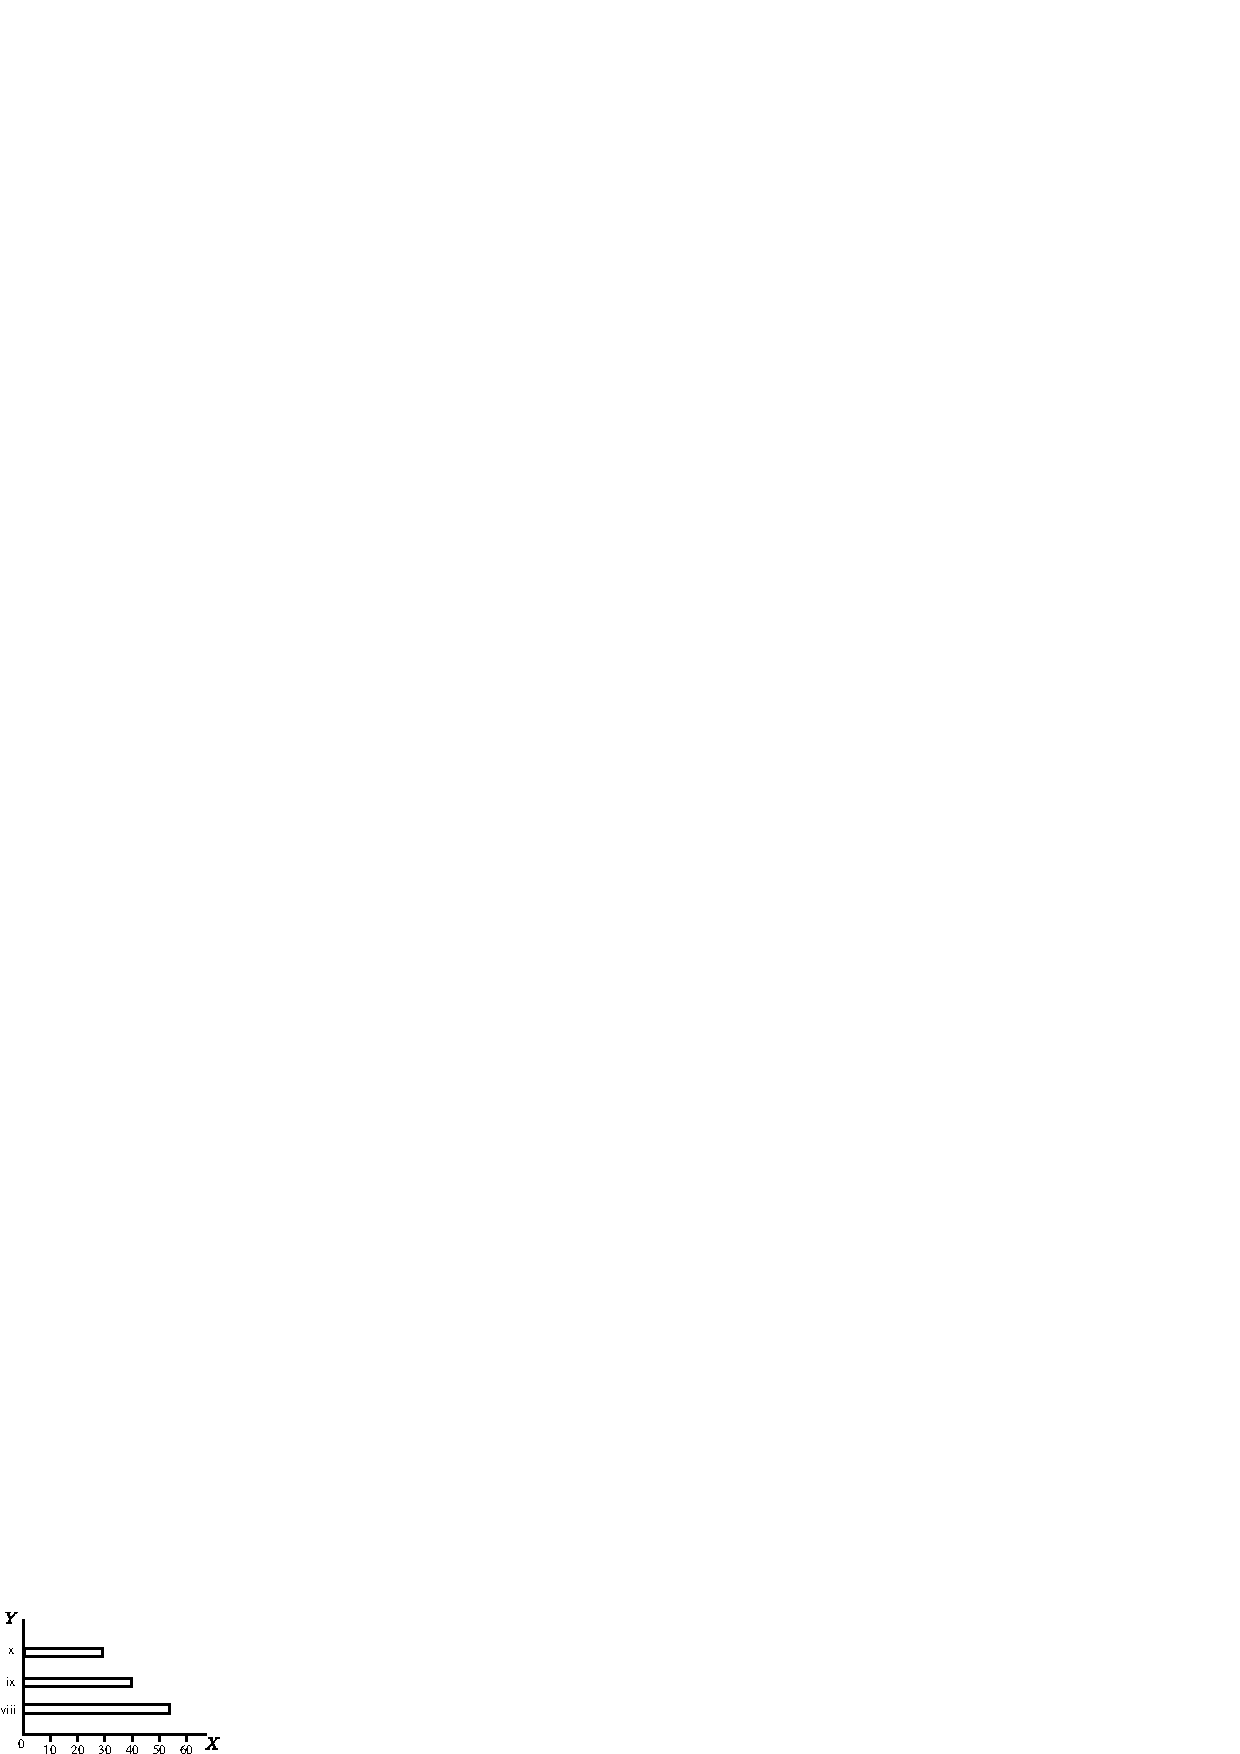
\includegraphics{figures/21.png}\\
\textbf{ಸಭಾಸೀನರಾಗಿರುವ ಪಾಠಶಾಲೆಯ ಅಧ್ಯಾಪಕ ಸಮೂಹ}\\[20pt]
\includegraphics{figures/20f.png}\\
\textbf{ವಿಶಾಲ ಸಭೆಯ ಇನ್ನೊಂದು ನೋಟ}
\end{tabular}
}

\eject
\thispagestyle{empty}

{\tabcolsep=0pt
\noindent
\begin{tabular}{>{\centering}p{11cm}}
\includegraphics{figures/22.png}\\
\textbf{ವೇದಸ್ವಸ್ತಿ - ವೇ॥  ಬ್ರ॥   ರಮೇಶ ಅಡಿಗರು ಮತ್ತು ವಿದ್ಯಾರ್ಥಿಗಳು}\\[20pt]
\includegraphics{figures/23.png}\\
\textbf{ಅಭಿವಂದನ ಗ್ರಂಥ ಬಿಡುಗಡೆಯ ಸಂದರ್ಭ}
\end{tabular}
}

\eject
\thispagestyle{empty}

{\tabcolsep=0pt
\noindent
\begin{tabular}{>{\centering}p{11cm}}
\includegraphics{figures/23a.png}\\
\textbf{ ಶ್ರೀಗಂಗಾಧರ ಭಟ್ಟರ ಕುರಿತಾದ ಸಾಕ್ಷ್ಯಚಿತ್ರದ\\ ಅನಾವರಣ ರಾಜಮಾತೆ ಪ್ರಮೋದಾ ದೇವಿಯವರಿಂದ}\\[20pt]
\includegraphics{figures/24a.png}\\
\textbf{ಸನ್ಮಾನದ ಪೂರ್ವಕ್ಷಣದಲ್ಲಿ ಆಚಾರ್ಯ ದಂಪತಿಗಳು}
\end{tabular}
}

\eject
\thispagestyle{empty}

{\tabcolsep=0pt
\noindent
\begin{tabular}{>{\centering}p{11cm}}
\includegraphics{figures/24.png}\\
\textbf{ಶ್ರೀಯುತರ ಧರ್ಮಪತ್ನೀ - ಶ್ರೀಮತಿ ಶೈಲಜಾರವರಿಗೆ\\ ಉಡಿತುಂಬಿದ ಶುಭಕ್ಷಣ}\\[20pt]
\includegraphics{figures/25a.png}\\
\textbf{ವಿದ್ಯಾರ್ಥಿಗಳ ಕನಸಿನ ಸನ್ಮಾನ ಸಂದರ್ಭ}
\end{tabular}
}

\eject
\thispagestyle{empty}

{\tabcolsep=0pt
\noindent
\begin{tabular}{>{\centering}p{11cm}}
\includegraphics{figures/25b.png}\\
\textbf{ವಿದ್ಯಾರ್ಥಿಗಳ ಕನಸಿನ ಸನ್ಮಾನ ಸಂದರ್ಭ}\\[20pt]
\includegraphics{figures/25c.png}\\
\textbf{ಸನ್ಮಾನ ಸಂದರ್ಭ}
\end{tabular}
}

\eject
\thispagestyle{empty}

{\tabcolsep=0pt
\noindent
\begin{tabular}{>{\centering}p{11cm}}
\includegraphics{figures/25h.png}\\
\textbf{ಸಮರ್ಪಿಸಿದ  ಶ್ರೀ ಎನ್.ಎಸ್. ರಾಮಭದ್ರಾಚಾರ್ಯರ \\ಭಾವಚಿತ್ರವನ್ನು  ಅವಲೋಕಿಸುತ್ತಿರುವ ಶ್ರೀಯುತರು}\\[20pt]
\includegraphics{figures/25j.png}\\
\textbf{ಸ್ವರ್ನವಲ್ಲೀ ಶ್ರೀಗಳಪರವಾಗಿ  ಗೌರವಪ್ರದಾನ -ವಿ ॥ ಶಂಕರ ಭಟ್ಟರಿಂದ}
\end{tabular}
}

\eject
\thispagestyle{empty}

{\tabcolsep=0pt
\noindent
\begin{tabular}{>{\centering}p{11cm}}
\includegraphics{figures/25d.png}\\
\textbf{ಸನ್ಮಾನಿತರಾದ ಆಚಾರ್ಯದಂಪತಿಗಳು}\\[20pt]
\includegraphics{figures/25e.png}\\
\textbf{ಡಾ ॥  ಪಿ.ಎನ್.ಶಾಸ್ತ್ರಿಗಳು ಮಾತನಾಡುತ್ತಿರುವ ಸಂದರ್ಭ}
\end{tabular}
}

\eject
\thispagestyle{empty}

{\tabcolsep=0pt
\noindent
\begin{tabular}{>{\centering}p{11cm}}
\includegraphics{figures/25f.png}\\
\textbf{ಡಾ ॥ ಆಳ್ವಾರ್ ರವರು ಅಧ್ಯಾಪಕ ಸಂಘದ ಪರವಾಗಿ ಮಾತನಾಡುತ್ತಿರುವುದು}\\[20pt]
\includegraphics{figures/32a.png}\\
\textbf{ಗಂಗಾಧರ ಭಟ್ಟರ ಸ್ನೇಹಿತರಾದ ಲಾಯರ್  ಶ್ರೀ ಕೆ.ಆರ್ ಶಿವಶಂಕರ್ ರವರು}
\end{tabular}
}

\eject
\thispagestyle{empty}

{\tabcolsep=0pt
\noindent
\begin{tabular}{>{\centering}p{11cm}}
\includegraphics{figures/25g.png}\\
\textbf{ವಿ ॥  ಉಮಾಕಾಂತ ಭಟ್ಟರು ಮಾತನಾಡುತ್ತಿರುವ ಸಂದರ್ಭ}\\[20pt]
\includegraphics{figures/26a.png}\\
\textbf{ರಾಜಮಾತೆ ಡಾ ॥  ಪ್ರಮೋದಾದೇವಿಯವರು ಮಾತನಾಡುತ್ತಿರುವ ಸಂದರ್ಭ}
\end{tabular}
}

\eject
\thispagestyle{empty}

{\tabcolsep=0pt
\noindent
\begin{tabular}{>{\centering}p{11cm}}
\includegraphics{figures/26b.png}\\
\textbf{ರಾಜಮಾತೆಯವರಿಗೆ ಗೌರವ ಸಮರ್ಪಣೆ}\\[20pt]
\includegraphics{figures/26.png}\\
\textbf{ ಶ್ರೀಯುತರು ಮಾತನಾಡುತ್ತಿರುವ ಸಂದರ್ಭ}
\end{tabular}
}

\eject
\thispagestyle{empty}

{\tabcolsep=0pt
\noindent
\begin{tabular}{>{\centering}p{11cm}}
\includegraphics{figures/27.png}\\
\textbf{ಸಭಾಧ್ಯಕ್ಷರಾದ ಡಾ ॥  ನಿರಂಜನ ವಾನಳ್ಳಿಯವರು\\ ಮಾತನಾಡುತ್ತಿರುವ ಸಂದರ್ಭ}\\[20pt]
\includegraphics{figures/28.png}\\
\textbf{ಕಾರ್ಯಕ್ರಮದ ಅಂತ್ಯಮಂಗಳ}
\end{tabular}
}

\eject
\thispagestyle{empty}

{\tabcolsep=0pt
\noindent
\begin{tabular}{>{\centering}p{11cm}}
\includegraphics{figures/28b.png}\\
\textbf{ಕಾರ್ಯಕ್ರಮದ ಅಂತ್ಯಮಂಗಳ ಸಂದರ್ಭದಲ್ಲಿ ಸಭೆ}\\[20pt]
\includegraphics{figures/30.png}\\
\textbf{ಸುಧರ್ಮಾದಿಂದ ಗೌರವಾರ್ಪಣೆ - ಗೌರವಸಂಪಾದಕರಾದ\\ಡಾ ॥ ಟಿ.ವಿ. ಸತ್ಯನಾರಾಯಣರವರು, ಡಾ ॥ ವಿ.ಡಿ. ಹೆಗಡೆಯವರು}
\end{tabular}
}

\eject
\thispagestyle{empty}

{\tabcolsep=0pt
\noindent
\begin{tabular}{>{\centering}p{11cm}}
\includegraphics{figures/29.png}\\
\textbf{ಹವ್ಯಕ ಸಂಘದ ಅಧ್ಯಕ್ಷರಾದ ವಿ ॥ ಲಕ್ಷ್ಮೀನಾರಾಯಣರಿಂದ ಗೌರವಾರ್ಪಣೆ}\\[20pt]
\includegraphics{figures/32.png}\\
\textbf{ಕುಟುಂಬ ವರ್ಗದೊಂದಿಗೆ ಆಚಾರ್ಯ ದಂಪತಿಗಳು}
\end{tabular}
}

\eject
\thispagestyle{empty}

{\tabcolsep=0pt
\noindent
\begin{tabular}{>{\centering}p{11cm}}
\includegraphics{figures/33.png}\\
\textbf{ ಶ್ರೀಯುತರ ಧರ್ಮಪತ್ನೀ ಶ್ರೀಮತಿ ಶೈಲಜಾರವರ\\ ತವರುಮನೆಯವರೊಂದಿಗೆ }\\[20pt]
\includegraphics{figures/31.png}\\
\textbf{ಪ್ರೀತಿಯ ವಿದ್ಯಾರ್ಥಿಸಮೂಹದೊಂದಿಗೆ ಶ್ರೀಗಂಗಾಧರ ಭಟ್ಟರು}
\end{tabular}
}
